\documentclass[10pt]{article}
\usepackage[utf8]{inputenc}
\usepackage[margin=0in,paperwidth=12in,paperheight=4in]{geometry}
\usepackage{tikz}
\usepackage{xcolor}
\usepackage{amsmath,amssymb}
\usetikzlibrary{shapes.geometric, arrows.meta, positioning, calc, backgrounds}
\pagestyle{empty}

\definecolor{bgdark}{HTML}{0F172A}
\definecolor{cardbg}{HTML}{1E293B}
\definecolor{bordercol}{HTML}{334155}
\definecolor{accentblue}{HTML}{38BDF8}
\definecolor{accentgreen}{HTML}{10B981}
\definecolor{accentorange}{HTML}{F59E0B}
\definecolor{accentpurple}{HTML}{A855F7}
\definecolor{accentred}{HTML}{EF4444}
\definecolor{accentcyan}{HTML}{06B6D4}
\definecolor{textwhite}{HTML}{F8FAFC}
\definecolor{textmuted}{HTML}{94A3B8}

\begin{document}
\noindent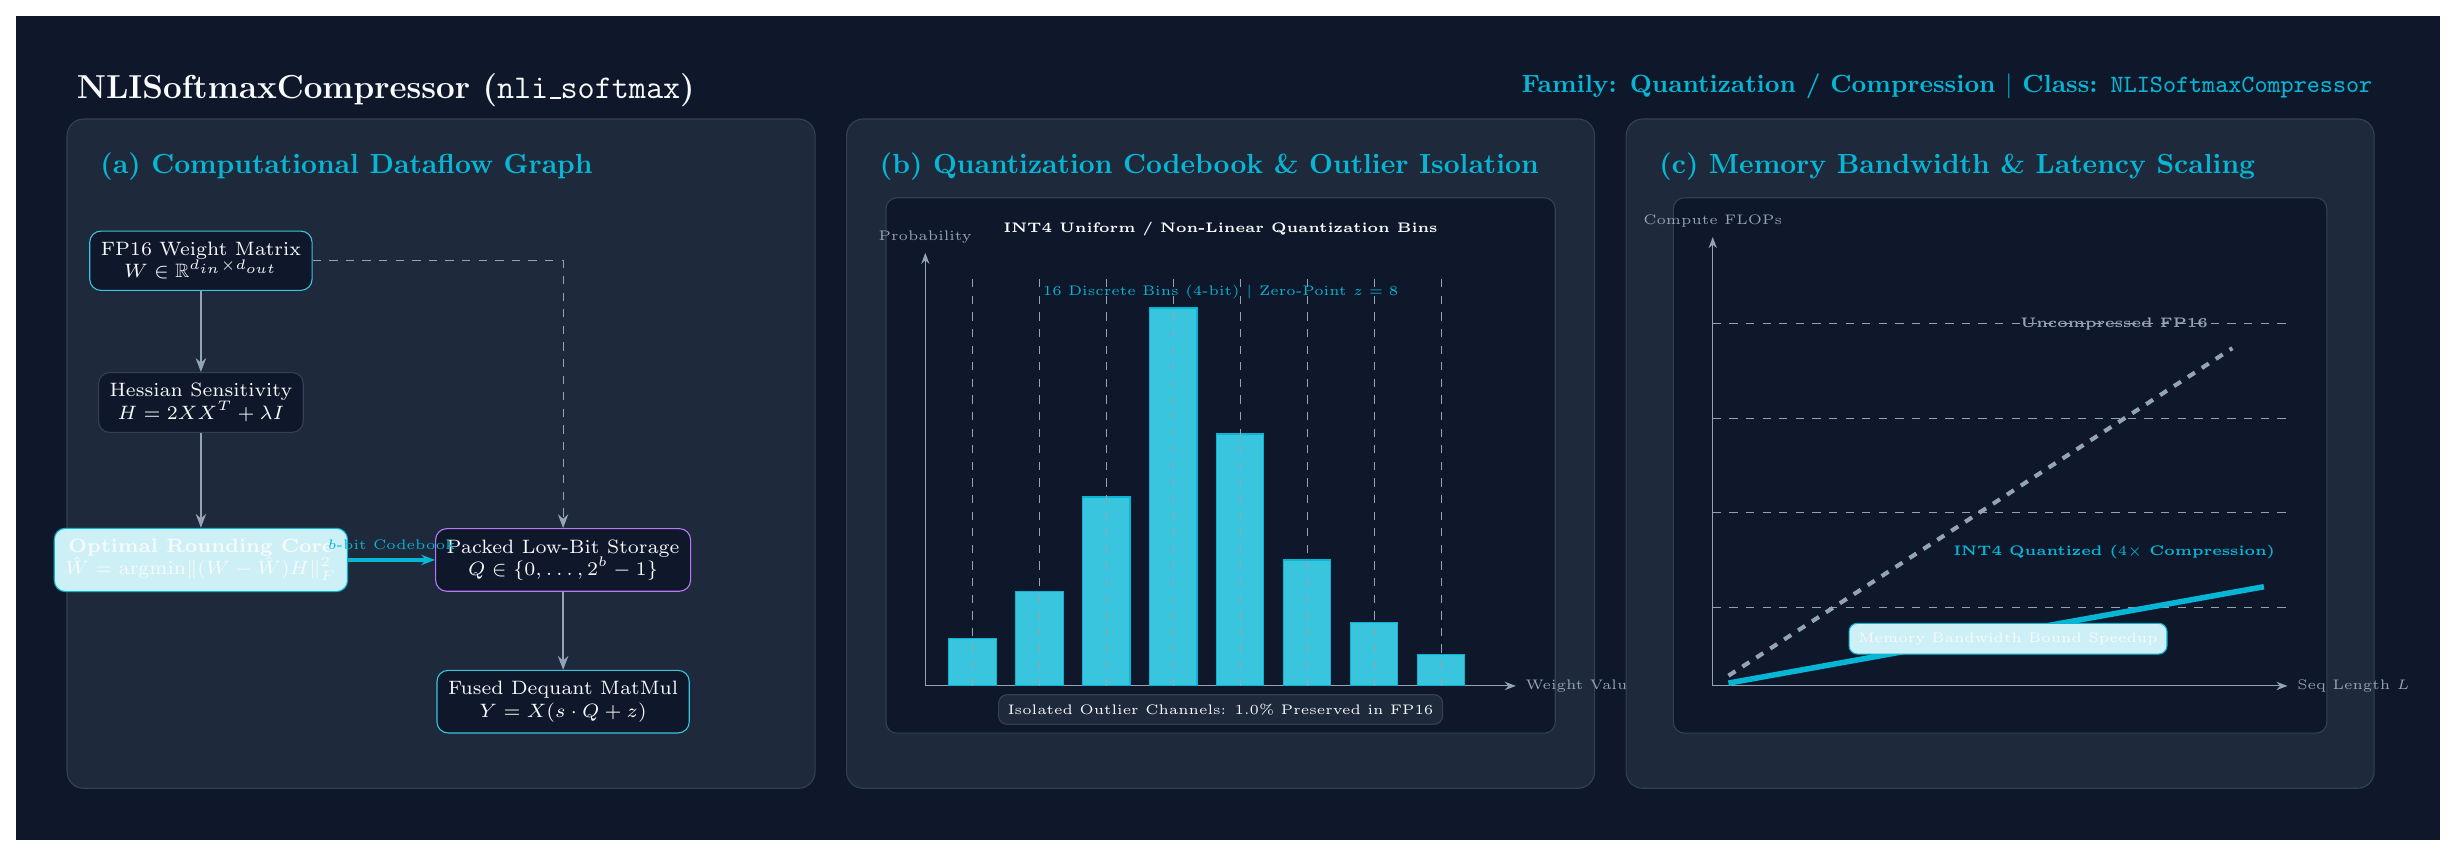
\begin{tikzpicture}[
    background rectangle/.style={fill=bgdark}, show background rectangle,
    scale=1.0, every node/.style={transform shape}
]

\clip (0,0) rectangle (30.48, 10.16);

% Title Header
\node[anchor=north west, text=textwhite, font=\large\bfseries] at (0.5, 9.7) {NLISoftmaxCompressor (\texttt{nli\_softmax})};
\node[anchor=north east, text=accentcyan, font=\small\bfseries] at (29.9, 9.7) {Family: Quantization / Compression $\mid$ Class: \texttt{NLISoftmaxCompressor}};

% Panel A: Computational Architecture
\draw[fill=cardbg, draw=bordercol, rounded corners=6pt] (0.5, 0.5) rectangle (10.0, 9.0);
\node[anchor=north west, text=accentcyan, font=\bfseries\normalsize] at (0.8, 8.7) {(a) Computational Dataflow Graph};

\node[draw=accentcyan!80, fill=bgdark, rounded corners=4pt, text=textwhite, font=\scriptsize, align=center, inner sep=4pt] (inp) at (2.2, 7.2) {FP16 Weight Matrix\\$W \in \mathbb{R}^{d_{in} \times d_{out}}$};
\node[draw=bordercol, fill=bgdark, rounded corners=4pt, text=textwhite, font=\scriptsize, align=center, inner sep=4pt] (proj) at (2.2, 5.4) {Hessian Sensitivity\\$H = 2 X X^T + \lambda I$};
\node[draw=accentcyan, fill=accentcyan!20, rounded corners=4pt, text=textwhite, font=\scriptsize\bfseries, align=center, inner sep=4pt] (core) at (2.2, 3.4) {Optimal Rounding Core\\$\hat{W} = \mathrm{argmin} \|(W - \hat{W})H\|_F^2$};
\node[draw=accentpurple!80, fill=bgdark, rounded corners=4pt, text=textwhite, font=\scriptsize, align=center, inner sep=4pt] (gate) at (6.8, 3.4) {Packed Low-Bit Storage\\$Q \in \{0, \dots, 2^b-1\}$};
\node[draw=accentcyan!80, fill=bgdark, rounded corners=4pt, text=textwhite, font=\scriptsize, align=center, inner sep=4pt] (outp) at (6.8, 1.6) {Fused Dequant MatMul\\$Y = X (s \cdot Q + z)$};

        \draw[-{Stealth[length=5pt]}, textmuted, line width=1pt] (inp) -- (proj);
        \draw[-{Stealth[length=5pt]}, textmuted, line width=1pt] (proj) -- (core);
        \draw[-{Stealth[length=5pt]}, accentcyan, line width=1.2pt] (core) -- (gate) node[midway, above, text=accentcyan, font=\tiny] {$b$-bit Codebook};
        \draw[-{Stealth[length=5pt]}, textmuted, line width=1pt] (gate) -- (outp);
        \draw[-{Stealth[length=5pt]}, dashed, textmuted] (inp) -| (gate);
        

% Panel B: Structural Pattern & Dynamics
\draw[fill=cardbg, draw=bordercol, rounded corners=6pt] (10.4, 0.5) rectangle (19.9, 9.0);
\node[anchor=north west, text=accentcyan, font=\bfseries\normalsize] at (10.7, 8.7) {(b) Quantization Codebook \& Outlier Isolation};
\draw[draw=bordercol, fill=bgdark, rounded corners=4pt] (10.9, 1.2) rectangle (19.4, 8.0);
\node[text=textwhite, font=\tiny\bfseries] at (15.15, 7.6) {INT4 Uniform / Non-Linear Quantization Bins};
\draw[-{Stealth[length=4pt]}, textmuted] (11.4, 1.8) -- (18.9, 1.8) node[right, font=\tiny] {Weight Value};
\draw[-{Stealth[length=4pt]}, textmuted] (11.4, 1.8) -- (11.4, 7.3) node[above, font=\tiny] {Probability};
\draw[fill=accentcyan!80, draw=accentcyan] (11.70, 1.8) rectangle (12.30, 2.40);
\draw[dashed, textmuted] (12.00, 1.8) -- (12.00, 7.0);
\draw[fill=accentcyan!80, draw=accentcyan] (12.55, 1.8) rectangle (13.15, 3.00);
\draw[dashed, textmuted] (12.85, 1.8) -- (12.85, 7.0);
\draw[fill=accentcyan!80, draw=accentcyan] (13.40, 1.8) rectangle (14.00, 4.20);
\draw[dashed, textmuted] (13.70, 1.8) -- (13.70, 7.0);
\draw[fill=accentcyan!80, draw=accentcyan] (14.25, 1.8) rectangle (14.85, 6.60);
\draw[dashed, textmuted] (14.55, 1.8) -- (14.55, 7.0);
\draw[fill=accentcyan!80, draw=accentcyan] (15.10, 1.8) rectangle (15.70, 5.00);
\draw[dashed, textmuted] (15.40, 1.8) -- (15.40, 7.0);
\draw[fill=accentcyan!80, draw=accentcyan] (15.95, 1.8) rectangle (16.55, 3.40);
\draw[dashed, textmuted] (16.25, 1.8) -- (16.25, 7.0);
\draw[fill=accentcyan!80, draw=accentcyan] (16.80, 1.8) rectangle (17.40, 2.60);
\draw[dashed, textmuted] (17.10, 1.8) -- (17.10, 7.0);
\draw[fill=accentcyan!80, draw=accentcyan] (17.65, 1.8) rectangle (18.25, 2.20);
\draw[dashed, textmuted] (17.95, 1.8) -- (17.95, 7.0);
\node[text=accentcyan, font=\tiny] at (15.15, 6.8) {16 Discrete Bins ($4$-bit) $\mid$ Zero-Point $z=8$};
\node[draw=bordercol, fill=cardbg, rounded corners=3pt, text=textwhite, font=\tiny] at (15.15, 1.5) {Isolated Outlier Channels: 1.0\% Preserved in FP16};

% Panel C: Complexity / Scaling Profile
\draw[fill=cardbg, draw=bordercol, rounded corners=6pt] (20.3, 0.5) rectangle (29.8, 9.0);
\node[anchor=north west, text=accentcyan, font=\bfseries\normalsize] at (20.6, 8.7) {(c) Memory Bandwidth \& Latency Scaling};

\draw[draw=bordercol, fill=bgdark, rounded corners=4pt] (20.9, 1.2) rectangle (29.2, 8.0);
\draw[-{Stealth[length=4pt]}, textmuted] (21.4, 1.8) -- (28.7, 1.8) node[right, font=\tiny, text=textmuted] {Seq Length $L$};
\draw[-{Stealth[length=4pt]}, textmuted] (21.4, 1.8) -- (21.4, 7.5) node[above, font=\tiny, text=textmuted] {Compute FLOPs};

\foreach \y in {2.8, 4.0, 5.2, 6.4} {
    \draw[dashed, bordercol!50] (21.4, \y) -- (28.7, \y);
}

        \draw[color=textmuted, line width=1.5pt, domain=21.6:28.0, dashed] plot (\x, {1.8 + 0.65*(\x-21.4)});
        \node[text=textmuted, font=\tiny\bfseries] at (26.5, 6.4) {Uncompressed FP16};
        \draw[color=accentcyan, line width=2pt, domain=21.6:28.4] plot (\x, {1.8 + 0.18*(\x-21.4)});
        \node[text=accentcyan, font=\tiny\bfseries] at (26.5, 3.5) {INT4 Quantized ($4\times$ Compression)};
        \node[draw=accentcyan, fill=accentcyan!20, rounded corners=3pt, text=textwhite, font=\tiny] at (25.15, 2.4) {Memory Bandwidth Bound Speedup};
        

\end{tikzpicture}
\end{document}
